%# -*- coding:utf-8 -*-
\documentclass[12pt,a4paper]{article}

\usepackage{buaa_paper}
\usepackage{fix-cm}


\schoolname{北京航空航天大学中法工程师学院}
\title{硕士学位论文文献综述}
\papertitle{基于词表分解优化的循环神经网络语言模型的研究}
\specialty{工业工程}
\studentnumber{ZY1624134}
\researcharea{自然语言处理}
\advisor{荣文戈~~副教授}
\author{是黎彬}
\date{2017 年 12 月 14 号}

\begin{document}

\maketitle



\addcontentsline{toc}{section}{摘要}
\keywords{大词表问题;词表分解;循环神经网络语言模型;自然语言处理}
{Over-large Vocabulary;\ Vocabulary Factorization;\ RNN Language Model;\ Natural Language Processing}

\begin{abstract_ch}
语言模型在自然语言处理领域起着非常重要的作用,该性能的好坏直接影响例如机器翻译和语音识别等很多任务的发展。随着循环神经网络的提出以及应用于语言模型上,计算机对人类语言的建模更加精确,但是也带来模型训练和运行速度都下降。尤其是当文本数据的数量急剧增长,单词的词表会变得巨大,这直接导致计算消耗十分大,包括计算复杂度太高所引起的运行耗时以及模型参数量太大所引起的内存占用过于庞大。为了解决这些问题,历史上人们开发了很多技术与模型,这些方法可以被分为三类:基于采样的近似算法,基于词表分解的算法,基于字母级别的编码模型。这些方法在一定程度上能缓解那些问题,但各自仍然存在一些缺陷。

本文首先概述语言模型的主要发展历史,详细阐述核心的建模方法——循环神经网络及其变种,解释大词表问题带来的重大挑战,列出了语言模型任务的国内外通用的标准数据集。然后上述所说的三大类前沿技术将会被总结分析优缺点,并重点讨论了基于词表分解的方法。最后,通过总结前人的方法,本文列出几个未来发展方向。
\end{abstract_ch}
\newpage
\begin{abstract_en}
Language model is a fundamental component in the field of neural language processing; its performance has direct influence on many tasks, e.g., machine translation and automatic speech recognition. With the propose of Recurrent Neural Network (RNN) and its inclusion in language model, language modeling by computer becomes more accuracy, yet producing the in-efficiency in the model’s training and operating. Especially when the text corpus growths explosively, vocabulary will become so huge that it causes both high computational complexity, which make it time-consuming to train as well as to infer, and excessive model size, which means the huge memory footprint. To tackle these problems, many techniques and models have been developed, mainly categorized as: sampling-based approximation, character level-based models, and vocabulary factorization-based methods.

In this paper we first review the development of the language model, containing the detail introduction of recurrent neural network and its variants, the explanation of the problem of over-large vocabulary, and some standard datasets. Afterwards, we explore those three kinds of advanced methods and analyze their merit and demerit. Finally, by summarizing the previous researches, we list some possible directions and the future works.

\end{abstract_en}
\newpage
\tableofcontents
\newpage

\section{论文选题的背景与意义}
\label{sec:intro}
近年来,互联网技术的快速发展,尤其是各大社交网络平台技术日趋完善,为人们营造了一个便于交流的世界。于是,在全球范围内互联网用户数量在不断增加,用户之间的交流、用户对互联网产品的评论以及各种信息的共享,这造成互联网上的数据爆炸式增长。其中,文本数据是用户信息传递的载体,如何从文本数据中自动挖掘有用的信息便成了一个各大互联网公司研究的热点。由此,对无标注的文本语言进行建模(Language Modeling, LM)就成了文本数据挖掘的一项非常重要的基础工作,很多文本挖掘应用场景,如信息检索 \cite{Jin:2002:TLM:564376.564386}、 机器翻译 \cite{DBLP:conf/naacl/BaltescuB15}、 语音识别 \cite{DBLP:conf/interspeech/SakSB14},都需要以语言模型为基本模块。因此,此研究课题是具有很强的实用价值和研究意义的。

在深度学习的概念提出之前,统计语言模型(Statistical Language Model, SLM) 是一种主要的对语言建模的方法,又称为N元语言模型(N-gram model \cite{DBLP:journals/csl/ChenG99}。自2006 年Hinton 提出深度学习(Deep Learning, DL)以来 \cite{hinton2006reducing},将深度学习应用于自然语言处理(Natural Language Processing, NLP)任务中已经成为自然语言处理界的趋势,尤其是在语言模型中的应用。研究者提出可以用神经网络(Neural Network, NN)对语言进行建模,包括前馈神经网络模型(Feed-Forward Neural Network, FFNN)\cite{DBLP:conf/nips/BengioDV00} 和循环神经网络模型(Recurrent Neural Network, RNN)\cite{DBLP:conf/interspeech/MikolovKBCK10}。其中,RNN 由于其特殊的网络结构能够将当前词的历史信息存储起来,并作为当前词预测的依据。该结构克服了N-gram语言模型无法利用距离当前词较远的词的信息。此外,在RNN 对一个词序列进行建模时,离散的词被映射到连续稠密的词嵌入(Word Embedding)空间,在这低维空间进行计算学习词序列的特征来学习词与词之间的依赖关系。因此,循环神经网络语言模型(Recurrent Neural Network Language Model, RNNLM)在模型困惑度(Perplexity, PPL)和词识别率上都取得了最好的结果 \cite{DBLP:conf/icassp/MikolovKBCK11}。

尽管RNNLM已经取得了重大的成功,但该模型仍然存在着很多难点,其中一个最为显著的问题是词表过大(Over-large vocabulary)的问题 \cite{DBLP:conf/interspeech/ChenWLGW14}。对此,由于语言模型旨在学习人类语言的模式,那么这意味着用于训练模型的人类语料越大,那么语言模型越能拟合语言模式并能因此模型生成的文本更像人说的语句一样。于是为了让模型更好的学习,这就不可避免的使得语料库数据量不断增长。词表过大的问题将会对RNNLM造成两个方面的巨大挑战:1)高计算复杂度(Computational complexity) \cite{DBLP:conf/acl/ChenGA16};2)庞大的模型参数量(Model size) \cite{DBLP:conf/nips/LiQYHL16}。

为了强调这些挑战的严峻性,在此列举一个例子来对此进行分析。One Billion Words (OBW)数据集是一个近年来公开的训练语言模型的语料数据集,它包含约80 万个不同的词,是一个典型的能够测试模型能否胜任词表过大这个问题的数据集。如果我们考虑一个标准的RNNLM,其中词嵌入向量的维度和RNN中的隐层的维度都设置为1024,并且在计算机中用32位浮点数去储存这些数据,那么通过计算可知该模型的大小达到7GB。 如此巨大的模型对于当前12GB的图形处理元件(Graphics Processing Units, GPUs)是极其困难的,甚至当训练时候增大每一批次的数据量,该GPUs已经无法处理该模型了。此外,通过一些基础实验发现,该模型的训练非常耗时,甚至要花费1个月的时间才能训练好。由此可见词表过大对于RNNLM 是一个巨大的且亟待解决的问题。因此探讨研究语言模型的大词表问题,是目前理论应用到实际过程中必须要克服的问题,也是值得研究和探讨的问题。

%因此探讨研究语言模型的大词表问题,是目前理论应用到实际过程中必须要克服的问题,也是值得研究和探讨的问题。为了克服这个问题,历史上研究者们做了很多尝试并开发了一系列的方法。我们讨论了三个不同方向的方法:一类是基于采样技术的近似方法(Sampling-based Approximation)\cite{DBLP:journals/tnn/BengioS08,DBLP:journals/jmlr/GutmannH12};一类基于字符级别(Char-level)的建模加速方法 \cite{DBLP:conf/aaai/KimJSR16}; 最后一类是基于词表分解(Vocabulary Factorization)的方法 \cite{DBLP:conf/icassp/Goodman01,DBLP:conf/icassp/MikolovKBCK11}。


\section{国内外研究现状及发展动态}

\subsection{N-gram 语言模型}
语言模型可以对一段文本的概率进行估计,对信息检索 \cite{Jin:2002:TLM:564376.564386}、 机器翻译 \cite{DBLP:conf/naacl/BaltescuB15}、 语音识别 \cite{DBLP:conf/interspeech/SakSB14} 等任务有着重要的作用。
形式化讲,统计语言模型的作用是为一个长度为$m$ 的字符串确定一个概率分布 $P(w_1;w_2;\cdots;w_m)$ ,表示其存在的可能性,其中$w_1$ 到$w_m$ 依次表示这段文本中的各个词。一般在实际求解过程中,通常采用下式计算其概率值:
\begin{equation}
\label{equ:lm}
\begin{split}
P(w_1;w_2; \cdots;w_m) &= P(w_1) P(w_2|w_1) P(w_3|w_1;w_2)\cdots P(w_i | w_1;w_2;\cdots;w_{i-1}) \\
&\cdots P(w_m | w_1;w_2;\cdots;w_{m-1})
\end{split}
\end{equation}
在实践中,如果文本的长度较长,公式 \ref{equ:lm} 右部$\cdots P(w_m | w_1;w_2;\cdots;w_{m-1}) $  的估算会非常困难, 因为出现$w_1;w_2;\cdots;w_{m-1};w_{m}$ 的语段非常少,进而该模型的稀疏性特别严重。因此,研究者们提出使用一个简化模型:n 元模型(n-gram model)。在n 元模型中估算条件概率时,距离大于等于n 的上文词会被忽略,也就是对上述条件概率做了以下近似:
\begin{equation}
\label{equ:approx}
P(w_i | w_1;w_2;\cdots;w_{i-1})  \approx P(w_i | w_{i-(n-1)};\cdots;w_{i-1})
\end{equation}
当$n = 1$ 时又称一元模型(unigram model),公式\ref{equ:approx} 右部会退化成$P(w_i)$,此时,整个句子的概率为:
\begin{equation}
P(w_1;w_2; \cdots;wm) = P(w_1)P(w_2) \cdots P(w_m)
\end{equation}
从式中可以知道,一元语言模型中,文本的概率为其中各词概率的乘积。也就是说,模型假设了各个词之间都是相互独立的,文本中的词序信息完全丢失。因此,该模型虽然估算方便,但性能有限。

当n = 2 时又称二元模型(bigram model),将n 代入公式\ref{equ:approx} 中,右部为P$(w_i|w_{i-1})$。 常用的还有n = 3 时的三元模型(trigram model),使用$P(w_i |w_{i-2};w_{i-1})$ 作为近似。这些方法均可以保留一定的词序信息 \cite{DBLP:journals/csl/ChenG99}。

\subsection{前馈神经网络语言模型}
N-gram语言模型的一个显著缺陷是:基于 \ref{equ:approx} 式,新词和低频词难以得到有效的概率统计。基于此,人们发明了各种平滑算法,如discount, back-off, interpolation 等 \cite{DBLP:conf/interspeech/2009,DBLP:journals/csl/ZhouL99}。 这些方法在一定程度上改善了n-gram 在低频词上的性能,但基于模型本身的缺陷,这一困难始终无法从根本上解决。

随着神经网络的兴起,人们开始尝试利用神经网络构造语言模型。与n-gram 不同,神经网络对参数进行高度共享,因此对低频词具有天然的平滑能力。神经网络语言模型(Neural Network Language Model, NNLM) 的最早由Bengio 等人在2001年提出\cite{DBLP:conf/nips/BengioDV00}, 近年来一些学者开始展开这方面的研究,并取得一系列成果,如\cite{DBLP:conf/acl/BaroniDK14,DBLP:journals/sigkdd/BellK07,DBLP:journals/pami/BengioCV13,DBLP:journals/tnn/BengioSF94}, 但总体而言, 对NNLM的研究还处在起步阶段。
具体而言,NNLM通过一个多层感知网络(MultiLayer Perceptron, MLP)来计算 \ref{equ:approx} 式中概率。
\begin{figure}
  \centering
  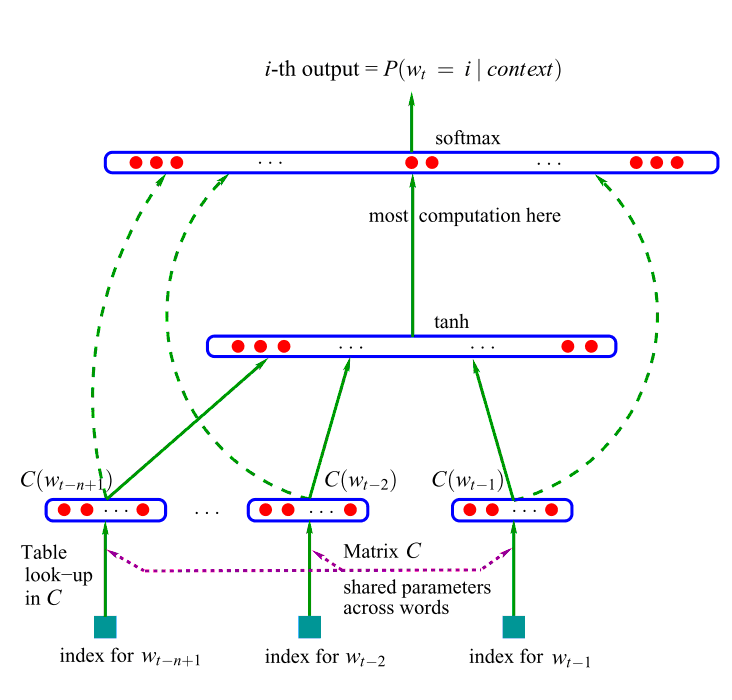
\includegraphics[width=0.7\linewidth]{./figures/nplm.png}
  \caption{前馈神经网络语言模型}\label{fig:nplm}
\end{figure}
图 \ref{fig:nplm} 给出一个典型的 NNLM 语言模型。神经网络语言模型采用普通的三层前馈神经网络结构,其中第一层为输入层。Bengio 提出使用各词的词向量作为输入以解决数据稀疏问题,因此输入层为词$w_{i-(n-1)}; \cdots;w_{i-1} $ 的词向量的顺序拼接:
\begin{equation}\label{equ:we}
  x = [e(w_{i-(n-1)}; \cdots ; e(w_{i-2}); e_{(w_{i-1})}]
\end{equation}
当输入层完成对上文的表示x 之后,模型将其送入剩下两层神经网络,依次得到隐藏层$h$ 和输出层$y$:
\begin{equation}\label{equ:all_nplm}
\begin{split}
h =& tanh(b(1) + Hx) \\
y =& b(2) +Wx + Uh
\end{split}
\end{equation}
其中 $H \in \mathbb{R}^{|h| \times (n-1)|e|}$ 为输入层到隐藏层的权重矩阵,$U \in \mathbb{R}^{|\mathrm{V}|\times (n-1)|h|}$ 为隐藏层到输出层的权重矩阵,$ |\mathrm{V}|$ 表示词表的大小,$|e|$ 表示词向量的维度,$|g|$ 为隐藏层的维度。$b(1),b(2)$ 均为模型中的偏置项。矩阵$W \in \mathbb{R}^{|\mathcal{V}|\times (n-1)|e|}$ 表示从输入层到输出层的直连边权重矩阵。由于$W$ 的存在,该模型可能会从非线性的神经网络退化成为线性分类器。Bengio 等人在文中指出,如果使用该直连边,可以减少一半的迭代次数;但如果没有直连边,可以生成性能更好的语言模型。因此在后续工作中,很少有使用输入层到输出层直连边的工作,下文也直接忽略这一项。如果不考虑$W$ 矩阵,整个模型计算量最大的操作,就是从隐藏层到输出层的矩阵运算$Uh$,后续的模型均有对这一操作的优化, 这部分内容将在下一节介绍。


\subsection{循环神经网络语言模型}
\label{sec:rnnlm}
Mikolov等人提出的循环神经网络语言模型(Recurrent Neural Network based Language Model,RNNLM)则直接对$P(w_i | w_1;w_2;\cdots;w_{i-1}) $ 进行建模,而不使用公式 \ref{equ:approx} 对其进行简化\cite{mikolov2012statistical,DBLP:conf/interspeech/MikolovKBCK10} 。因此,RNNLM 可以利用所有的上文信息,预测下一个词,其模型结构如图 \ref{fig:rnnlm} 所示。

\begin{figure}
  \centering
  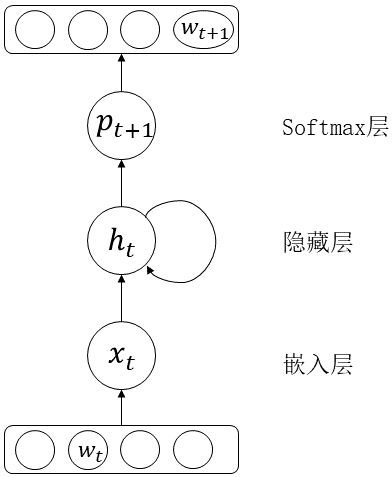
\includegraphics[width=0.85\linewidth]{./figures/rnnlm.png}
  \caption{循环神经网络语言模型(RNNLM)模型结构图}\label{fig:rnnlm}
\end{figure}

RNNLM 的核心在于其隐藏层的算法:
\begin{equation}
\label{equ:rnn}
h(i) =\phi(e(w_i) +Wh(i -1))
\end{equation}
其中,$\phi$非线性激活函数。但与NNLM 不同,RNNLM 并不采用n 元近似,而是使用迭代的方式直接对所有上文进行建模。在公式\ref{equ:rnn} 中,h(i) 表示文本中第$i$ 个词$w_i$ 所对应的隐藏层,该隐藏层由当前词的词向量$e(w_i)$ 以及上一个词对应的隐藏层$h(i -1)$ 结合得到。

隐藏层的初始状态为$h(0)$,随着模型逐个读入语料中的词$w_1;w_2; \cdots $, 隐藏层不断地更新为$h(1);h(2); \cdots$ 。根据公式\ref{equ:rnn},每一个隐藏层包含了当前词的信息以及上一个隐藏层的信息。通过这种迭代推进的方式,每个隐藏层实际上包含了此前所有上文的信息,相比NNLM 只能采用上文n 元短语作为近似,RNNLM 包含了更丰富的上文信息,也有潜力达到更好的效果。RNNLM 的输出层计算方法与NNLM 的输出层一致。


\section{研究目标和研究内容}
\subsection{大词表问题分析}
\label{sec:vocab}
本文已经在第\ref{sec:intro}章节通过举例凸显出词表过大的问题,此小节简单解释为什么词表过大会造成灾难性的问题。第\ref{sec:rnnlm}节已经详细地介绍了循环神经网络语言模型的(Recurrent Neural Network Language Model, RNNLM)的结果与原理,由此可知其建模过程为,RNNLM 使用一个嵌入层(Embedding Layer)将词映射至一个用稠密向量空间的表示词嵌入(Word Embedding),紧接着使用一个隐层(Hidden Layer)来对这些词嵌入进行编码,最后使用归一化指数函数(Softmax)进行预测下一个词在词表中的位置。

在这个过程中,词表的大小与Embedding Layer直接相关,因为所有在词表中的词都要通过Embedding Layer来获取向量表示才能进行后续的计算。我们可以简单的计算一下就可以发现其中的问题,假设一个数据集上的词表为$\mathcal{V}$,那么这个词表大小可以表示为${|\mathcal{V}|}$,另外不妨设词嵌入的向量维度为${|D|}$,那么这个Embedding Layer 的参数量为${\mathcal{O}(|\mathcal{V}| \times |D|)}$。当词嵌入维度${|D|}$不变,如果词表过大的话,那么这个参数量是十分巨大的,这是一个非常直观的影响。

同时,这个建模过程还直接影响Softmax,导致预测过程十分耗时。前面说过,Softmax 是用来依据当前词以及当前词的上下文的综合信息来预测下一个词的函数,这个预测也可以被看作是一个多分类(Multi-label Classification)任务。Softmax 预测的公式为如下:
\begin{equation}\label{eq:softmax}
\begin{split}
	p(w)=\frac{\exp(z_w)}{\sum_{w^{'}\in\mathcal{V}} {\exp(z_{w^{'}})}}
\end{split}
\end{equation}
其中$w$是指要在词表$\mathcal{V}$中预测的词,$z_w$指相关词的非归一化的激励分值。但是公式中的归一化项${Z=\sum_{w^{'}\in\mathcal{V}} {\exp(z_{w^{'}})}}$ 需要遍历整个词表上对所有词的预测分值进行求和,会带来非常高的计算量并使得模型低效。对于一个大小为${|\mathcal{V}|}$ 的词表,Softmax的计算复杂度等于${\mathcal{|\mathcal{V}|}}$,那么当词表过大的时候,该模块的计算量就会巨大。

为了尝试解决这些问题,很多种方法被开发出来,他们可以被分成3类:基于采样的近似,基于字符级别的建模以及基于词表分解的预测。以下章节对这三类方法一一介绍。
\subsection{基于采样近似方法}
由上一小节介绍可知,模型的计算复杂度很大程度上来源于Softmax中的归一化项,每一个词的预测都需要在整个词表范围内做求和计算,这个计算量必然庞大。针对这个问题,研究者们就发明了一些采样方法来对此做一些近似,这就是基于采样的近似方法(Sampling-based Approximation)。重要性采样(Importance Sampling, IS)\cite{DBLP:conf/aistats/BengioS03}、自适应重要性采样(Adaptive Importance Sampling, AIS)\cite{DBLP:journals/tnn/BengioS08}、噪声对比估计(Noise Contrastive Estimation)\cite{DBLP:journals/jmlr/GutmannH12,DBLP:conf/icml/MnihT12}以及负采样(Negative Sampling)\cite{DBLP:journals/corr/abs-1301-3781}都是属于这一类的方法。这些方法的核心思想是通过采样技术从词表中选取一部分的词来近似计算Softmax预测以及该函数的梯度。其中,最具代表性的且比较稳定的方法是NCE,下文对该方法做一个详细的介绍。
NCE是一种Mnih和Teh发明的比重要性采样更稳定的采样方法,该方法不是直接估计某个词的概率值,相反,它的学习目标是训练一个模型能够将正确的目标词和采样出来的噪声区分开。于是待解决的问题就由从词表中预测出正确的词语的复杂问题化简为一个二分类问题,即训练一个分类器尝试将正确的词语与所有其他噪声样本中的错误词区分出来,如图所示。
\begin{figure}
  \centering
  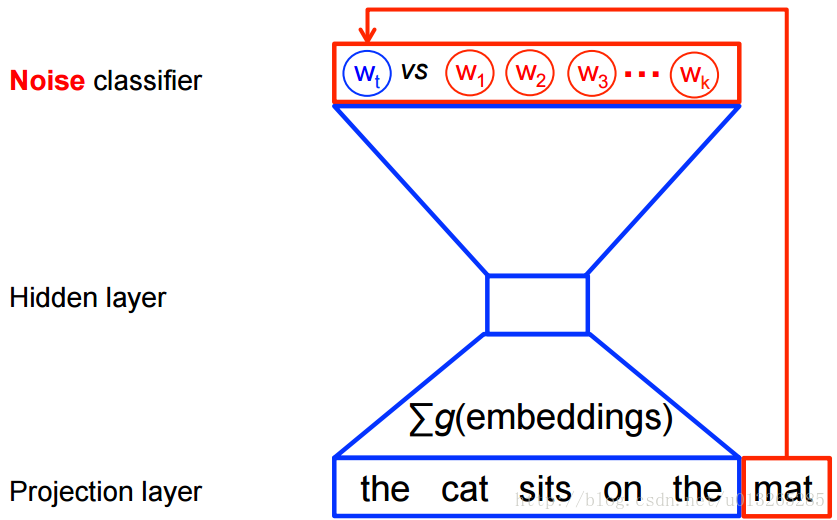
\includegraphics[width=0.6\linewidth]{./figures/nce.png}
  \caption{噪声对比估计(NCE)}\label{fig:nce}
\end{figure}

对于每个词${w_i}$,它的前n个词${w_{t-1},\cdots,w_{t-n+1}}$表示为语境${c_i}$。 然后从含有噪声分布$Q$中生成$k$个噪声样本${\tilde{w}_{ik}}$,由于是一个二分类问题,那么可以标记正确词$w_i$为正样本${(y=1)}$,标记剩下的噪声词${\tilde{w}_{ik}}$为负样本${(y=0)}$。

于是按二分类常用的代价函数来训练:
\begin{equation}
J_\theta = -\sum\limits_{w_i \in \mathcal{V}}{[\log P(y=1|w_i, c_i) + k\mathbb{E}_{\tilde{w}_{ik}}[\log P(y=0|\tilde{w}_{ik}, c_i)]]}
\end{equation}
其中$\mathbb{E}$表示期望,那么该公式可以简化为:
\begin{equation}
J_\theta = -\sum\limits_{w_i \in \mathcal{V}}{[\log P(y=1|w_i, c_i) + \sum\limits_{j=1}^k{\log P(y=0|\tilde{w}_{ik}, c_i)}]}
\end{equation}
剩下的是要推导出该公式中的概率值来:已知所有预测词都是从两个分布中采样得到的,其中正样本可以看做是从训练集${P_{train}}$中采样,而负样本是从噪声分布$Q$ 中采样得到,因此概率可以看做是两部分的按比组合为:
\begin{equation}
P(y,w|c) = \frac{1}{k+1} P_{train}(w|c) + \frac{k}{k+1}Q(w)
\end{equation}
于是,一个词来自训练集样本的概率为:
\begin{equation}
\begin{split}
P(y=1|w,c) &=  \frac{\frac{1}{k+1} P_{train}(w|c)}{\frac{1}{k+1} P_{train}(w|c) + \frac{k}{k+1}Q(w)} \\
           &= \frac{P_{train}(w|c)}{P_{train}(w|c) + kQ(w)} \\
           &= \frac{\frac{\exp(z_w)}{Z}}{\frac{\exp(z_w)}{Z} + kQ(w)}
\end{split}
\end{equation}
其中,$Z$为归一化项,也就是公式\ref{eq:softmax}里的归一化项。这一项的计算量非常大,而NCE 采用一个小技巧来避免,NCE的作者Mnih 和Teh把$Z$的值固定为1,他们认为这个近似对模型不会造成太大的影响。于是该公式就变为,
\begin{equation}
  P(y=1|w,c) = \frac{\exp(z_w)}{\exp(z_w) + kQ(w)}
\end{equation}
带入上述的代价函数中,最终得到NEC的代价函数:
\begin{equation}
J_\theta = -\sum\limits_{w_i \in \mathcal{V}}{\left[\log \frac{\exp(z_w)}{\exp(z_w) + kQ(w)} + \sum\limits_{j=1}^k{\log \frac{\exp(z_{\tilde{w}})}{\exp(z_{\tilde{w}}) + kQ(\tilde{w})}}\right]}
\end{equation}

NCE方法有完美的理论证明:随着噪声样本$k$的数量增加,NCE导数趋近于Softmax 函数的梯度。Mnih 和Teh认为抽取25个噪声样本就足以到达Softmax函数的效果,而速度能提升大约45 倍,这是一个非常好的提升\cite{DBLP:conf/icml/MnihT12}。
\subsection{基于字符级别建模方法}
\begin{figure}
  \centering
  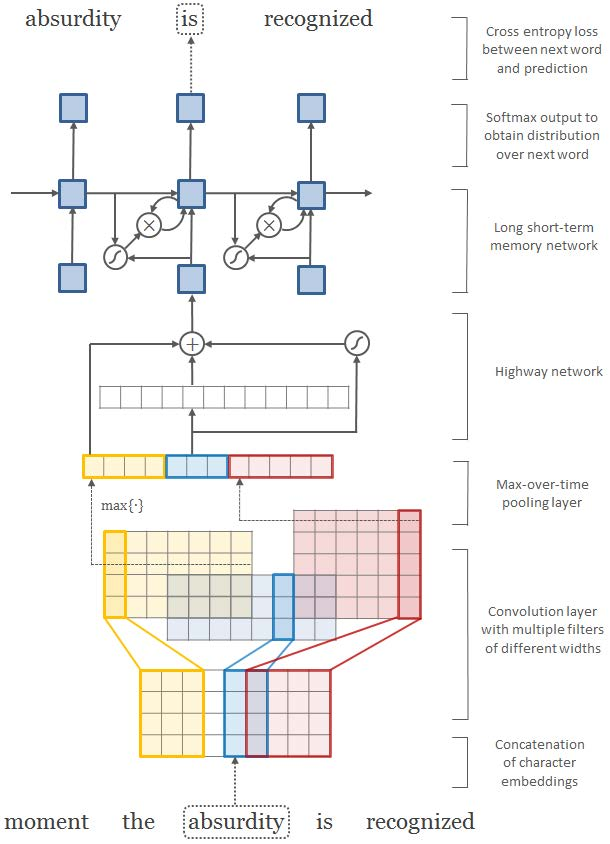
\includegraphics[width=0.4\linewidth]{./figures/CharCNN.jpg}
  \caption{基于字符级别建模的语言模型}\label{fig:charcnn}
\end{figure}
本文在第\ref{sec:vocab}章节分析了由词表过大带来的问题,那么就意识到需要针对这个大词表做一些处理。对此,Kim发明了CharCNN\cite{DBLP:conf/aaai/KimJSR16},与之前的方法在词级别建模的方法相比,该方法利用英语单词的特殊性——尽管词的数量非常庞大,但是所有词都由26个字母组成。如果能在对字母级别进行建模,那模型的大小能得到缩减。CharCNN就是用字符级别的输入代替原始的词级别的输入,那么这能将词嵌入层的参数从原始的${\mathcal{O}(|\mathcal{V}| \times |\mathcal{D}|)}$缩减至${\mathcal{O}(|Char| \times |\mathcal{D}|)}$,其中${|Char|}$指的是字符的数量。其完整的建模过程在图\ref{fig:charcnn}中列出。

尽管该方法能利用字符数量少的特性来将模型的大小缩减,但是仍然存在着一些问题,比如字符级别只能被用在嵌入层,而Softmax层的参数量没有变,因为它扔需在词表范围内去做预测,那么它还要遭受Softmax层在大词表上预测低效性的困扰。此外,这一方法只能应用于西方语言建模问题上,而对于中文字,这个方法就失效了。

\subsection{基于词表分解预测方法}
\label{sec:vocab_facto}
\begin{figure}
  \centering
  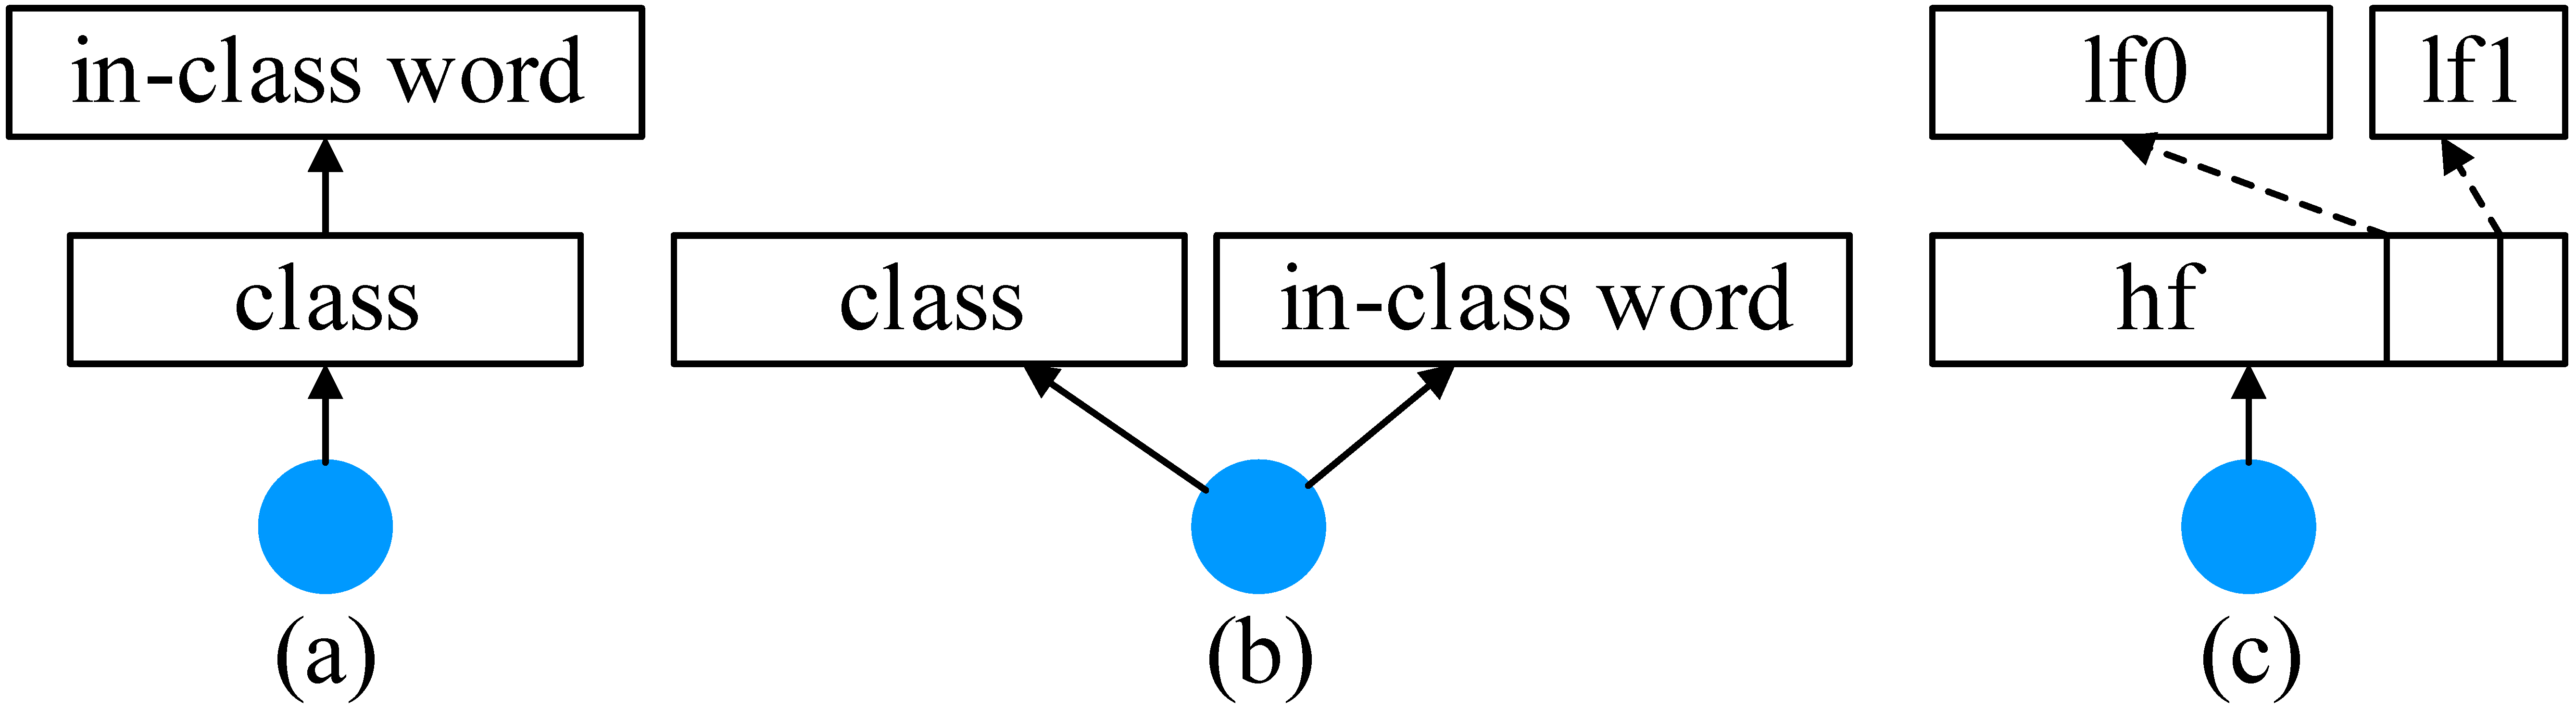
\includegraphics[width=0.65\columnwidth]{./figures/softmax3.png}
  \caption{三种不同的在Softmax层中词类组织关系的结构。(a) 层级组织结构;(b) 并列组织结构;(c) 分片组织结构,图中hf表示高频(high frequency),而lf表示低频(low frequency),其中lf0和lf1是根据词的低频程度把词分配起来。另外,在图中蓝色的单元表示包含历史信息和当前输入词信息的隐层,这一点对于这三种方法都一致。}
  \label{fig:softmax}
\end{figure}
\subsubsection{Hierarchical Softmax}
\begin{figure}
  \centering
  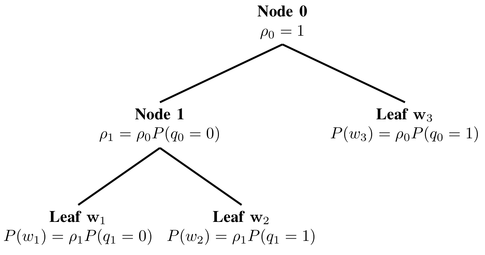
\includegraphics[width=0.65\columnwidth]{./figures/thsm.jpg}
  \caption{树结构层次Softmax}
  \label{fig:thsm}
\end{figure}
与前两类的方法不同的是,基于词表分解的方法是在词级别输入上进行建模的,而且该方法在预测的时候也没有近似。该类方法使用完整的词表,并且利用词表的结构性和层级性以及条件概率把原来的词的一步预测分解成多步预测问题。这一类的方法有很多,包括基于双层结构Softmax(Class-based Hierarchical Softmax, cHSM)的方法\cite{DBLP:conf/icassp/Goodman01,DBLP:conf/icassp/MikolovKBCK11,DBLP:conf/acl/ChenGA16,DBLP:conf/icml/GraveJCGJ17} 和基于树层级结构Softmax(Tree-based Hierarchical Softmax, tHSM)的方法\cite{DBLP:conf/aistats/MorinB05,DBLP:conf/nips/MnihH08}。

对于cHSM来说,他们的核心想法是要把通过传统的Softmax进行词的预测方法分裂成两个步骤。原来的Softmax 是直接把一个词从词表中预测出来,而cHSM是先预测这个词属于的类别,然后再在这个类别中预测出具体哪个词,公式可以表示为如下:
\begin{equation}
\label{eq:cHSM}
\begin{split}
	p(w|h)=p(c|h)p(w|c,h)
\end{split}
\end{equation}
其中$h$表示词$w$的上下文信息。如果我们把词表$\mathcal{V}$中的所有词分配到${\sqrt{|\mathcal{V}|}}$个平衡的类中(平衡意味着每个类里面的单词数量是一致的),那么该计算复杂度就由原来的${\mathcal{O}(|\mathcal{V}|)}$ 缩减到${\mathcal{O}(\sqrt{|\mathcal{V}|})}$。

cHSM从一开始由Goodman(2001)发明出来一直到现今仍然有相近的方法提出,其核心的加速原理一直没用变。从深度学习流行之前Goodman 用最大熵语言建模(Maximum Entropy Language Model)方式\cite{DBLP:conf/icassp/Goodman01}到目前流行的循环神经网络的建模方式\cite{DBLP:conf/asru/MikolovDPBC11};以及无论该方法中类的组织关系作何变化,包括层级组织结构\cite{DBLP:journals/jmlr/BengioDVJ03}、 并列组织结构\cite{DBLP:conf/icassp/MikolovKBCK11}和分片组织结构\cite{DBLP:conf/acl/ChenGA16},这三种组织结构的示意图如图\ref{fig:softmax} 所示。
\begin{itemize}
  \item 层级组织结构:该结构就是一个最经典的两层的层级Softmax,先预测词的类别,然后在该类别中预测词,如图\ref{fig:softmax}中(a)所示;
  \item 并列组织结构:该结构将词的类下标和类中词下标合并在一起,然和同时预测这两个下标,如图\ref{fig:softmax}中(b)所示;
  \item 分片组织结构:该结构认为文本中的词会根据词出现频率而具有不同的重要性,词频越大,那么该词就越重要。基于这个想法,该结构先根据词频大小将词表划分成多个片段,然后给每个片段赋予不同的参数量,如果片段词频大,那么就要赋予更多的参数去学习他们的特征。其结构如图\ref{fig:softmax} 中(c) 所示。
\end{itemize}

对于tHSM,它可以被看作是cHSM的延伸。tHSM扩展了cHSM的思想,把Softmax层继续分裂,直到把原始的Softmax分裂成一个树结构(Tree)。所有的词都列在在这棵树的叶子节点(Leaf Node)上,而这棵树的中间节点表示词表的深层次结构,如图\ref{fig:thsm}所示。如果考虑用一个平衡的二叉树结构来组织词类的结构关系,那么这种tHSM的计算复杂度又继续减小至${\mathcal{O}(\log |\mathcal{V}|)}$。

\subsubsection{LightRNN}
\begin{figure}
  \centering
  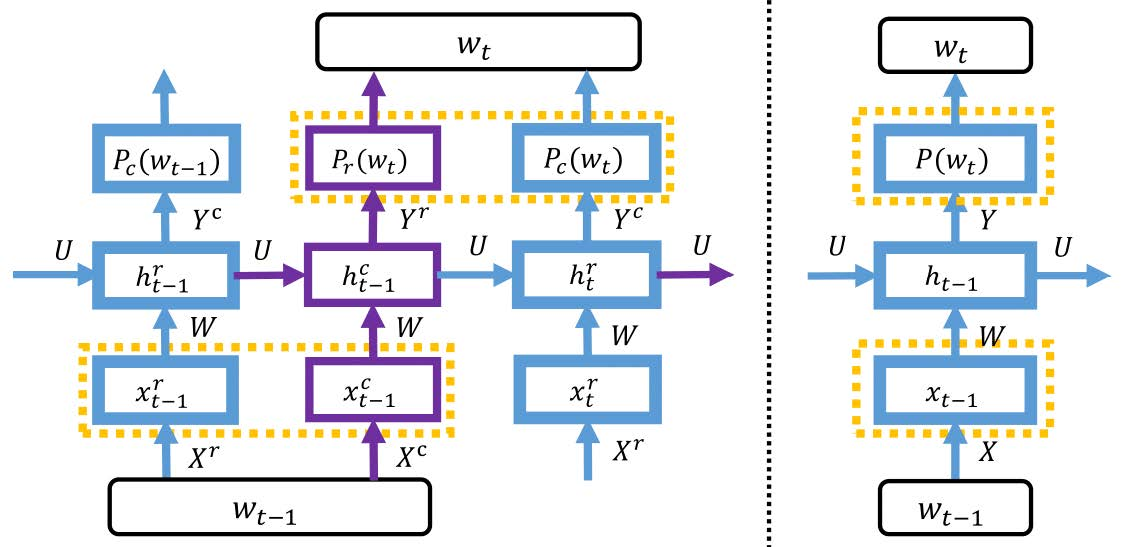
\includegraphics[width=0.65\columnwidth]{./figures/lightrnn.jpg}
  \caption{LightRNN}
  \label{fig:lightrnn}
\end{figure}
前面介绍的方法要么专门用来减小计算复杂度以加速,要么专门用来缩减模型的大小,却没有一个模型同时能在来两方面同时进行优化的。LightRNN方法的提出不仅能减小模型计算复杂度,还能大幅度缩减模型的大小\cite{DBLP:conf/nips/LiQYHL16}。基于该想法,LightRNN提出一个2-Component shared embedding,将词分配到一个二维的词表里面。词表所有相同行的词共享一个行向量,所有相同列的词共享一个列向量。而一个词由其对应的行向量与列向量联合表示。这样,我们就仅需要${2\sqrt{|\mathcal{V}|}}$个向量来表示词表中所有的词。对于每个用行标和列标表示的词来说,LightRNN更改了原始的RNN 结构来对双标表示的词进行编码,其结构如图\ref{fig:lightrnn}。这种方法能够将词嵌入层和Softmax层的维度降低至${\mathcal{O}(\sqrt{|\mathcal{V}|} \times |D|)}$ 和${\mathcal{O}(\sqrt{|\mathcal{V}|} \times |H|)}$。该方法的另一个值得学习的地方是将词交换问题变成一个最小费用最大流问题(Minimum Cost Maximum Flow, MCMF),并利用一个优化算法\cite{Preis1999}去解决这个问题。

\section{拟解决的关键问题及对应的研究路线}
\subsection{词聚类方法的研究}
\subsection{词表交换算法的研究}
\subsection{基于词表分解的建模方式研究}

\section{论文研究计划}
\begin{itemize}
  \item 2017年12月\~{}2018年1月
  \item 整理资料,学习深入研究词聚类方法
  \item 2018年2月\~{}2018年4月
  \item 深入研究词表交换算法
  \item 2018年5月\~{}2018年6月
  \item 深入研究基于词表分解的建模方式
  \item 2018年6月\~{}2018年7月
  \item 代码整合,实验验证与完善
  \item 2018年7月\~{}2018年8月
  \item 整理资料和论文撰写
\end{itemize}

\section{总结与展望}
本文首先介绍了语言模型的背景知识以及对语言模型进行深入研究的重要意义。然后,本文简要概述了语言模型的一发展历史,从一开始基于统计的N-gram语言模型,到深度学习被提出以来神经网络模型应用于语言模型使得语言模型的性能得到飞跃的提升,尤其是循环神经网络的引入,这触发了将循环神经网络应用于自然语言处理领域这一热潮。紧接着,本文从理论上分析循环神经网络语言模型的缺点,分析为何词表过大会带来灾难性的问题,并且详细的介绍了针对这个问题近几年学术界提出的新模型和新方法,本文把这些方法分成三大类,并对每一类方法都进行详细的阐述其原理,并解释为何这些方法能从一定角度上缓解词表过大的问题。

通过阅读大量的关于语言模型的文献,能够对现有的方法都有了一定的了解。下一步,我们将对这些方法进行总结与归纳,发现其中的一些问题,并尝试进行优化。尤其是词表分解这一类的方法,我们可以尝试去做一些优化。针对词表分解这一类的方法,我们已经酝酿了一些初步的想法,下一步是要将想法实践出来,通过实验去验证这些想法,并在这个过程中再去分析和总结,再优化我们的想法。
\newpage
\addcontentsline{toc}{section}{参考文献}
\bibliography{bibs}

\end{document}
